\begin{figure}
    % \centering
    % \begin{tikzpicture}
    %     \begin{axis}[view={40}{30}, axis lines=none]
    %         \addplot3[
    %             surf,
    %             colormap/cool,
    %             shader=flat,
    %             opacity=.6,
    %             domain=-2:2,
    %             domain y=-1:2,
    %             samples=10,
    %             clip=false
    %             ] {x^2 - y^2};
        
            
    %         \addplot3[
    %             color=red, thick, samples=5, smooth, samples y=0, domain=-0.5:-0.5
    %         ]
    %         ({x},   
    %         {0},  
    %         {x^2}   
    %         );
            
    %         \addplot3[
    %             color=red, thick, samples=5, smooth, samples y=0, domain=-0.5:-0.5
    %         ]
    %         ({2*x+1},   
    %         {0},  
    %         {x^2}   
    %         );

    %         \addplot3[
    %             color=red, thick, samples=5, smooth, samples y=0, domain=-0.5:-0.5
    %         ]
    %         ({-2*x+1},   
    %         {0},  
    %         {x^2}   
    %         );           
                
            
    %         \end{axis}
    %     \end{tikzpicture}

    \centering
    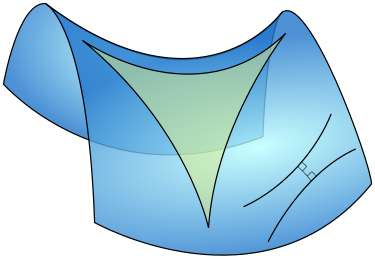
\includegraphics[width=0.3\textwidth]{figs/Hyperbolic_triangle.png}    
    \caption{Section of a hyperbolic space.}
    \label{fig:hyperbolicSpace}
\end{figure}


